
%
%  $Description: FRED Toolchain paper for RTAS 2008$
%
%  $Author: volgy $
%  $Date: 2007/10/09 15:20:59 $
%  $Revision: 1 $
%

\documentclass[times, 10pt,twocolumn]{article}
\usepackage{latex8}
\usepackage{times}
\usepackage{graphicx}

%\documentstyle[times,art10,twocolumn,latex8]{article}

%-------------------------------------------------------------------------
% take the % away on next line to produce the final camera-ready version
\pagestyle{empty}

%-------------------------------------------------------------------------
\begin{document}

\title{Towards a Model-based Toolchain for the \\
High-Confidence Design of Embedded Systems}

\author{P\'{e}ter V\"{o}lgyesi, G\'{a}bor Karsai,  Sandeep Neema, Harmon Nine, \\
Joseph Porter, Ryan Thibodeaux,  and J\'{a}nos Sztipanovits \\
Institute for Software Integrated Systems \\
Vanderbilt University\\
Nashville, TN 37235, USA \\
peter.volgyesi@vanderbilt.edu\\
}
\maketitle
\thispagestyle{empty}
\begin{abstract}
While design automation for hardware systems is quite advanced,
this is not the case for practical embedded systems. The current
state-of-the-art is to use a software modeling environment
and integrated development environment for code development and debugging, but
these rarely include the sort of automatic synthesis and
verification capabilities available in the VLSI domain. This paper
introduces concepts, elements, and some early prototypes for
an envisioned suite of tools for the development of embedded
software that integrates verification steps into the overall
process.
\end{abstract}

\Section{Introduction}
\section{Introduction}

High confidence embedded control system software designs often require formal 
analyses to ensure design correctness.  Detailed models of system behavior 
include numerous design concerns, such as controller stability, timing 
requirements, fault tolerance, and deadlock freedom.  Models for each of these
domains must together provide a consistent and faithful representation of the
potential problems an operational system would face.  This poses challenges 
for structural representation of models, as components and design
aspects are commonly tightly coupled.  The ESMoL language is built on a platform which provides inherent correctness properties for well-formed models.  The properties include functional determinism, deadlock freedom, and timing determinism.  We also rely on decoupling
methods such as passive control design (decoupling controller stability from
network effects) and time-triggered models of computation (decoupling timing 
and fault tolerance from functional requirements) and on compositional 
and incremental analysis to enable rapid prototyping in our design environment.  As design paradigms become more fully decoupled and analysis becomes faster (and therefore cheaper), we move closer to the goal of ``correct by construction'' model-based software 
development.

In compositional analysis for graphical software models, sometimes the nature of the analysis does not easily lead to a clean syntactic decomposition in the models.  Examples include end-to-end properties such as latency, and other properties which require the evaluation of particular connections spanning multiple levels of components.  One approach for dealing with such properties in hierarchical dataflow designs is the creation of interface data for each component which abstracts properties of that component.  Hierarchical schedulability models defined over dataflows are a particular example\cite{sched:shin} -- each composite task contains a resource interface characterizing the aggregate supply required to schedule the task and all of its children.  Extensions to the formalism allow the designer to efficiently and incrementally evaluate whether new tasks can be admitted to the design without recomputing the full analysis\cite{sched:easwaran}.  One goal is to see whether this approach can be generalized to other properties that do not easily fit the compositional structure of hierarchical designs.
 
One particular syntactic analysis problem concerns synchronous execution environments 
and system assembly.  In dataflow models of computation we are often concerned with 
so-called ``algebraic'' or delay-free processing loops in a design model.  Many
synchronous formalisms require the absence of delay-free loops in order to 
guarantee deadlock freedom \cite{moc:ltta} or timing determinism \cite{moc:sdf}.
This condition can be encoded structurally into dataflow modeling languages --
for example Simulink \cite{tools:mathworks} analyzes for algebraic loops and attempts to resolve them analytically.  In the Ptolemy dataflow design environment, such causality loops 
complicate scheduling requiring fixed-point iteration to ensure convergence of 
results\cite{tools:ptolemy2}. In our work we only consider the structural 
problem of loop detection in model-based distributed embedded system designs.

We propose a simple incremental cycle enumeration technique with the following
characteristics:

\begin{itemize}
\item The algorithm uses Johnson's simple cycle enumeration algorithm as its 
core engine\cite{cycles:johnson75}.  Johnson's algorithm is known to be 
efficient \cite{cycles:mateti76}.  We use cycle enumeration rather than simple
detection in order to provide useful feedback to the designers.
\item The algorithm exploits the component structure of hierarchical dataflow 
models to allow the cycle enumeration to scale up to larger models.   A small amount of interface data is created and stored for each component as the analysis processes the model hierarchy from the bottom up.  The interface data consists of a set of typed graph edges indicating whether dataflow paths exist between each of the component's input/output pairs.  Each component is evaluated for cycles using the interface data instead of the detailed dataflow connections of its child components.
\item   The interface data facilitates incremental analysis, as it also contains a flag to determine whether modifications have been made to the component.  We refer to the flag and the edges as an \emph{incremental interface} for the component.  This is consistent with the use of the concept in other model analysis domains, such as compositional scheduling analysis\cite{sched:easwaran}. In order for the incremental method to assist our development processes, the total runtime for all partial assessments of the model should be no greater than the analysis running on the full model.  Because the amount of interface data supporting the incremental analysis is small, the method should scale to large designs without imposing onerous data storage requirements on the model.
\item The technique will not produce false positive cycle reports, though it 
may compress multiple cycles into a single cycle through the interface abstraction.  Fortunately,
full cycles can be recovered from the abstract cycles through application
of the enumeration algorithm on a much smaller graph.
\end{itemize}

Zhou and Lee presented an algebraic formalism for detecting causality cycles
in dataflow graphs, identifying particular ports that participate in a cycle.
\cite{comp:causality}. Our work traverses the entire model and extracts all 
elementary cycles,
reporting all ports and subsystems involved in the cycle.
Our approach is also inspired by work from Tripakis et al, which 
creates a richer incremental interface for components to capture execution 
granularity as well as potential deadlock information\cite{moc:hsdf}.  
Their approach is lossless, in that it retains sufficient detail to faithfully represent dataflow structure and execution granularity.  It is much more complex in both model space and computation than our approach. Our formalism does not aim to pull 
semantic information forward into the interface beyond connectivity.  In that sense our approach is more general, as it could be applied to multiple 
model analysis problems in the embedded systems design domain.

The KPASSA model analysis tool described by Boucaron et al 
\cite{cycles:boucaron} performs task graph scheduling analysis for 
latency-insensitive synchronous designs.   Their formal model leans heavily on loop structures, and as such one component of their tool relies on an 
implementation of Johnson's cycle enumeration algorithm\cite{cycles:boucaron2}.  Their formal model is specific to a particular model of computation, and their application of cycle checking is only one small component of that solution.




\Section{The vision}

\begin{figure}
	\centering
   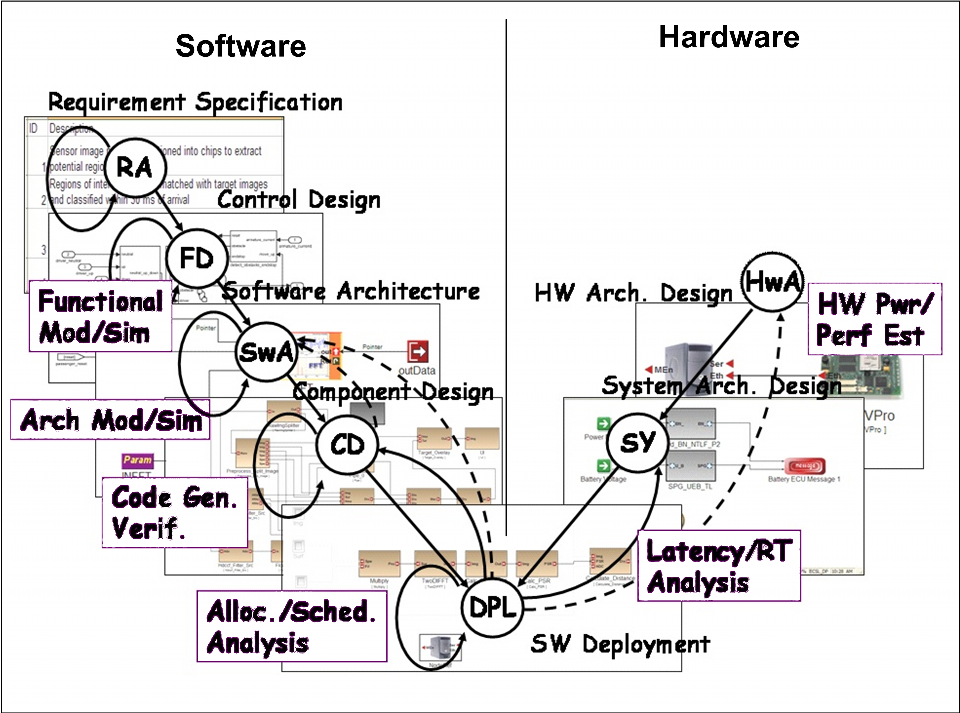
\includegraphics[width=0.65\columnwidth]{diagrams/vdiagram.png}
   \caption{Conceptual model of the toolchain: Development flow}
   \label{fig:vdiagram}
\end{figure}

In this work, we envision a sophisticated, end-to-end toolchain that supports not only construction but also the verification of the engineering artifacts (including software) for high-confidence applications. The development flow provided by the toolchain shall follow a variation of the classical V-model (with software and hardware development on the two branches), with some refinements added at the various stages. Fig. \ref{fig:vdiagram} illustrates this development flow.

Consider the general class of control system designs for use in a flight control system.  Sensors, actuators, and data networks are designed redundantly to mitigate faults.  The underlying hardware implements a variant of the time-triggered architecture (TTA)~\cite{kopetz:2001-22a}, which provides precise timing and reliability guarantees.  Safety-critical tasks and messages execute according to strict precomputed schedules to ensure synchronization between replicated components and provide fault mitigation and management.  Software implementations of the control functions must pass strict certification requirements which impose constraints on the software as well as on the development process.  

A modeling language to support this development flow must have several desired properties:  (1) the ability to capture the relevant aspects of the system architecture and hardware, (2) ability to ``understand'' (and import) functional models from existing design tools, (3) support for componentization of functional models, and (4) ability to model the deployment of the software architecture onto the hardware architecture. The ability to import existing models from functional modeling tools is not a deeply justified requirement, it is merely pragmatic.  EsMoL provides modeling concepts and capabilities that are highly compatible with AADL~\cite{AADL}.  The chief differences are that EsMoL aims for a simpler graphical entry language, a wider range of execution semantics, and most important model-enabled integration to external tools as described below.  Model exchange with AADL tools may be desirable in the future.  A simple sample design will introduce key points of our model-based development flow and illustrate language concepts.  

Our language design was influenced by two factors: (1) the MoC implemented by the platform and (2) the need for integration with legacy modeling and embedded systems tools. We have chosen Simulink/Stateflow as the supported ``legacy'' tool. As our chosen MoC relies on periodically scheduled time-triggered components, it was natural to use this concept as the basis for our modeling language and interpret the imported Simulink blocks as the implementation of these components. To clarify the use of this functionality, we import a Simulink design and select functional subsets which execute in discrete time, and then assign them to software components using a modeling language that has compatible (time-triggered) semantics. Communication links (signals) between Simulink blocks are mapped onto TTA messages passed between the tasks. The resulting language provides a componentized view of Simulink models that are scheduled periodically (with a fixed rate) and communicate using time-triggered messages.  Extensions to heterogeneous MoC-s is an active area of research.

\subsection{Requirements Analysis (RA)}

Our example will model a data network implementing a single sensor/actuator loop with a distributed implementation.  The sensors and actuators in the example are doubly-redundant, while the data network is triply-redundant.  Unlike true safety-critical designs, we will deploy the same functions on all replicas rather than requiring multiple versions as is often done in practice~\cite{DO178B}.  The sensors and actuators close a single physical feedback loop.  Specifying the physical system and particulars of the control functions are beyond the scope of this example as our focus is on modeling.

This example has an informal set of requirements, though our modeling language currently supports the formalization of timing constraints between sensor and actuator tasks.  Formal requirements modeling offers great promise, but in ESMoL requirements modeling is still in conceptual stages.  A simple sensor/actuator latency modeling example appears in a later section covering preliminary features for the language.

\subsection{Functional Design (FD)}

\begin{figure}
	\centering
   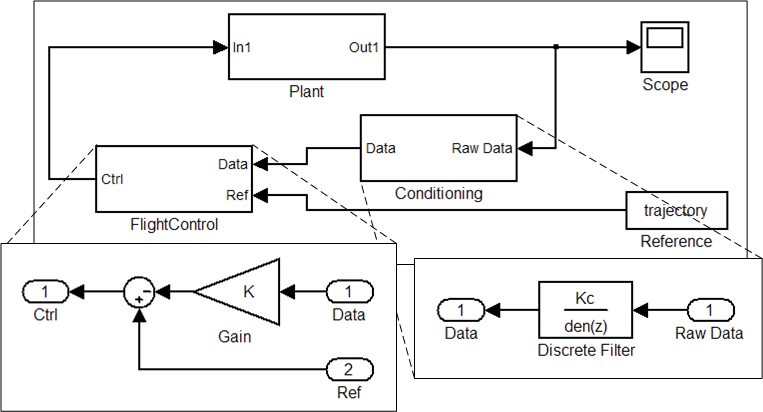
\includegraphics[width=0.65\columnwidth]{diagrams/sl_design.png}
   \caption{Simulink design of a basic signal conditioner and controller.}
   \label{fig:sl_design}
\end{figure}

Functional designs can appear in the form of Simulink/Stateflow models or as existing C code snippets.  ESMoL does not support the full semantics of Simulink. In ESMoL the execution of Simulink data flow blocks is restricted to periodic discrete time, consistent with the underlying time-triggered platform.  This also restricts the type and configuration of blocks that may be used in a design.  Continuous integrator blocks and sample time settings do not have meaning in ESMoL.  C code snippets are captured in ESMoL as well.  C code definitions are limited to synchronous, bounded-time function calls which will execute in a periodic task.

\begin{figure}
	\centering
   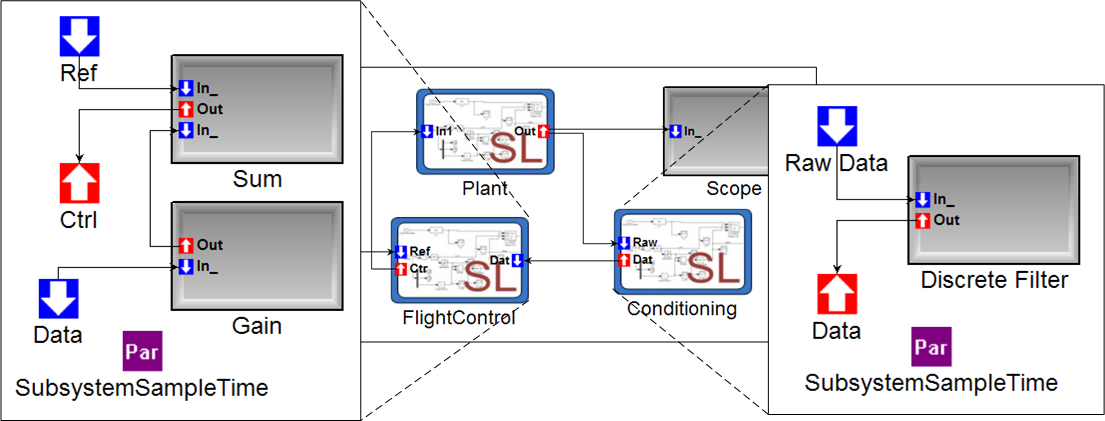
\includegraphics[width=0.9\columnwidth]{diagrams/esmol_design.png}
   \caption{ESMoL-imported functional models of the Simulink design.}
   \label{fig:esmol_design}
\end{figure}

Fig. \ref{fig:sl_design} shows a simple top-level Simulink design for our feedback loop along with the imported ESMoL model (Fig. \ref{fig:esmol_design}).  The ESMoL model is a structural replica of the original Simulink, only endowed with a richer software design environment and tool-provided APIs for navigating and manipulating the model structure in code.  A model import utility provides the illustrated function.

\subsection{Software Architecture (SwA)}

\begin{figure}
	\centering
   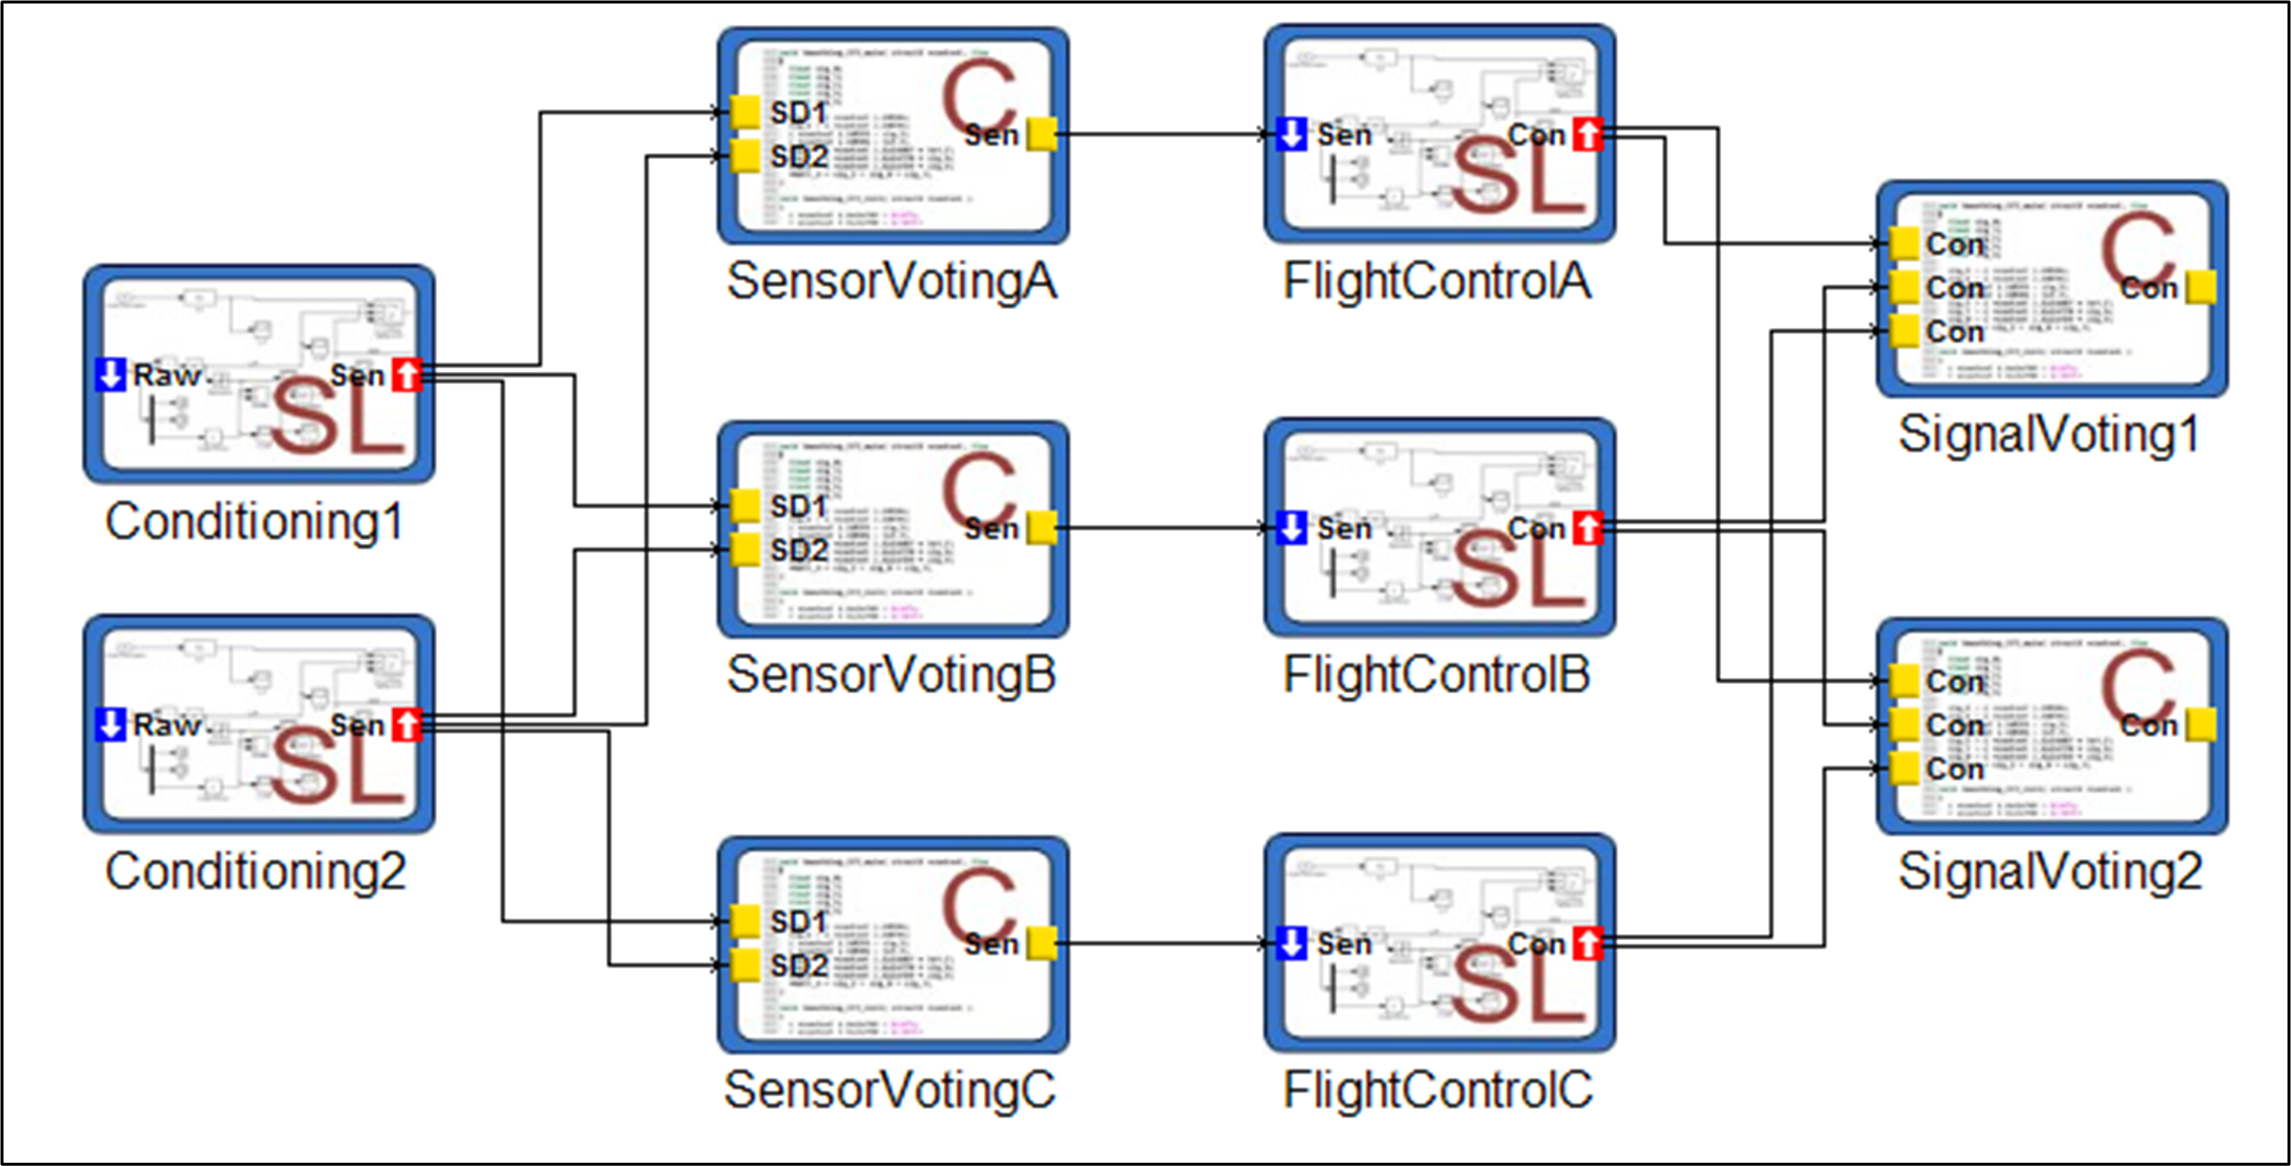
\includegraphics[width=0.7\columnwidth]{diagrams/tmr_arch.png}
   \caption{The architecture diagram defines logical interconnections, and gives finer control over instantiation of functional units.}
   \label{fig:tmr_arch}
\end{figure}

The software architecture model describes the logical interconnection of functional blocks.  In the architecture language a component may be implemented by either a Simulink Subsystem or a C function.  They are compatible at this level, because here their model elements represent the code that will finally implement the functions.  These units are modeled as blocks with ports, where the ports represent parameters passed into and out of C function calls.  The semantics for architecture model connections is that of sending and receiving messages using time-triggered communication.  

Fig. \ref{fig:tmr_arch} shows the architecture diagram for our TMR model.  Instances of the functional blocks from the Simulink model are augmented with C code implementing replicated data voting.

\subsection{Hardware Architecture (HwA)}

\begin{figure}
	\centering
   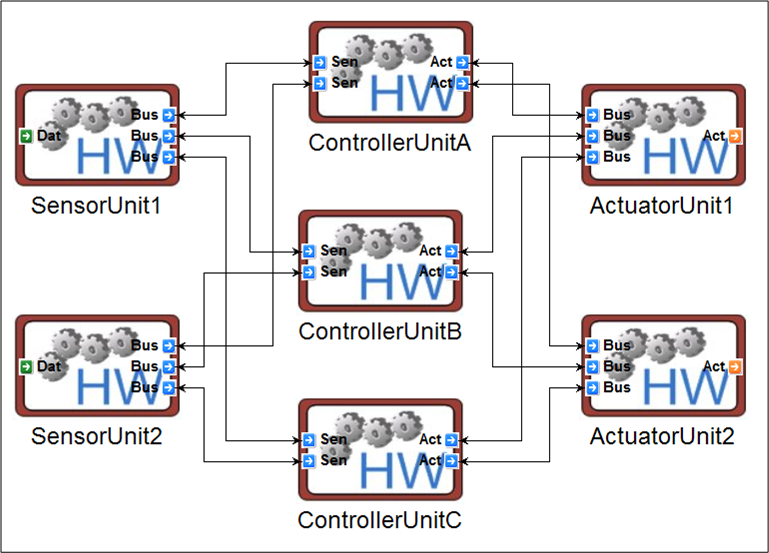
\includegraphics[width=0.75\columnwidth]{diagrams/tmr_hardware.png}
   \caption{Overall hardware layout for the TMR example.}
   \label{fig:tmr_hardware}
\end{figure}

Hardware configurations are explicitly modeled in the platform language.  Platforms are defined hierarchically as hardware units with ports for interconnections. Primitive components include processing nodes and communication buses.  Behavioral semantics for these networks come from the underlying time-triggered architecture.  The platform provides services such as deterministic execution of replicated components and timed message-passing.  Model attributes for hardware also capture timing resolution, overhead parameters for data transfers, and task context switching times.

\begin{figure}
	\centering
   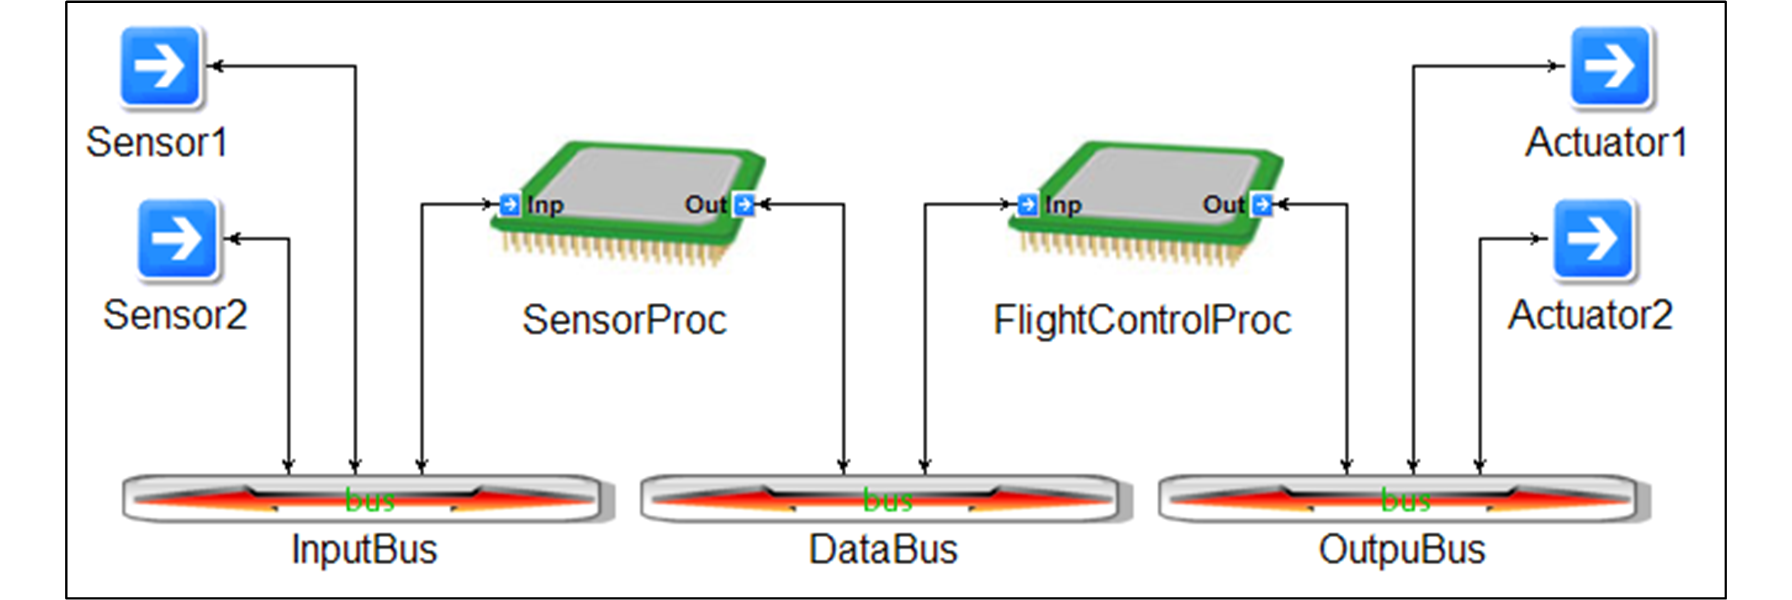
\includegraphics[width=0.8\columnwidth]{diagrams/platformex.png}
   \caption{Detail of hardware model for controller units.}
   \label{fig:platformex}
\end{figure}

Figs. \ref{fig:tmr_hardware} and \ref{fig:platformex} show model details for redundant hardware elements.  Each controller unit is a private network with two nodes and three independent data buses.
Sensor voting and flight control function instances will be deployed to the controller unit networks.

\subsection{Deployment Models (CD, SY, DPL)}

\begin{figure}
	\centering
   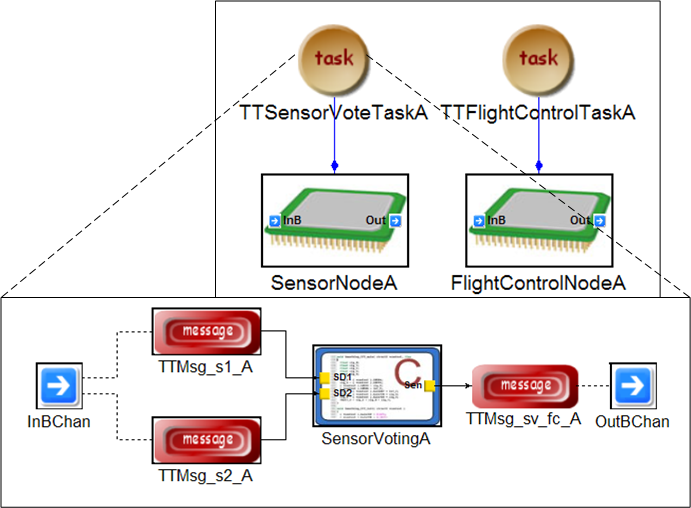
\includegraphics[width=0.55\columnwidth]{diagrams/tmr_deploy.png}
   \caption{Deployment model: task assignment to nodes and details of task definition.}
   \label{fig:tmr_deploy}
\end{figure}

A common graphical language captures the grouping of architecture components into tasks.  In ESMoL a task executes on a single processing node at a single periodic rate.  All components within the task execute synchronously.  Data sent between tasks takes the form of messages in the model.  Whether delivered locally (same processing node) or remotely, all inter-task messages are scheduled for delivery.  ESMoL uses logical execution time semantics found in time-triggered languages such as Giotto~\cite{henzinger01giotto} -- message delivery is scheduled after the deadline of the sending task, but before the release of the receiving tasks.  In the TT model of computation receivers assume that their data is available at task release time.  Tasks never block, but execute with whatever data is available each period.

Deployment concepts, tasks running on processing nodes and messages sent over data buses, are modeled as shown in Fig. \ref{fig:tmr_deploy}.  Most of the model elements shown here are actually references to elements defined in the architecture and platform models.  Model interpreters generate platform-specific code and analysis artifacts directly from the deployment models.

%%% OLD STUFF %%%%%%%%%%%%%%%%%%%%%%%%%%%%%%%%%%%%%%%%%%%%%%%%%%%%%%%%%%%%%%%%%%%%%%%%%%%%%



%\subsection{Code generators and synthesis tools}
%Model-based development is a high-level activity, i.e. programming with models instead of an algorithmic language. Therefore we need to generate executable code from the models. With proper infrastructure the generator could be more than just a model-to-code translator; it could be a code 'synthesizer' yielding low-level code from higher-level specifications. Synthesis differs from translation as it may search during the code generation process. For instance, on platforms with fixed-point arithmetic, the synthesizer could determine appropriate scaling factors for each operational step in a dataflow model based on known value ranges for inputs and outputs and the available fixed-point precision.

%Generating code from dataflow and Statechart models is a well-defined and solved problem, and there are many actual implementations. Code synthesis from higher-level models, however, is an active area of research with many open questions regarding code efficiency and correctness.

%\subsection{Verification and analysis}
%Verification and analysis are an inseparable part of the development process for high-confidence systems. There are many well-known verification techniques and tools; however, we must stress two concerns here: (1) verification tools often operate on models (i.e. abstractions of the system), not on detailed code and (2) verification results are meaningful only if model transformations from design models into analysis models or into code are correct: Properties must be carried over by the transformation with no addition of any artifacts extending behavior of the generated code beyond that of the model.

%Verification of model translators and construction of verification-based tools is an active area of research. Correctness of a model transformations is a very complex problem, but some early results indicate promising directions \cite{ananth:2006}: instead of proving correctness for a transformation in general, one can show that a particular instance of a transformation preserves the properties of interest and conclude that the properties hold for the input of the transformation.

%Another promising direction is a connection between models and the generated code. We are working on extending the code generator to carry forward model-level information to the generated code (as annotations) that provide help for the code-level verifier to check model-level properties on the code. This connection could potentially be used to improve performance, as the verifier could reason using higher-level abstractions than those immediately available from the code.  Other relevant work includes distributed modeling and verification tools like BIP~\cite{BasuBozgaSifakis07}, which strives for separation of concerns using a layered behavior model.


\Section{Elements of the toolchain}
Below, we describe the implemented elements of the toolchain. Figure \ref{fig:existing} illustrates the toolchain as it exists today, and it shows how the services needed (e.g. scheduling, code generation) are implemented by specific elements.

\begin{figure}[h]
   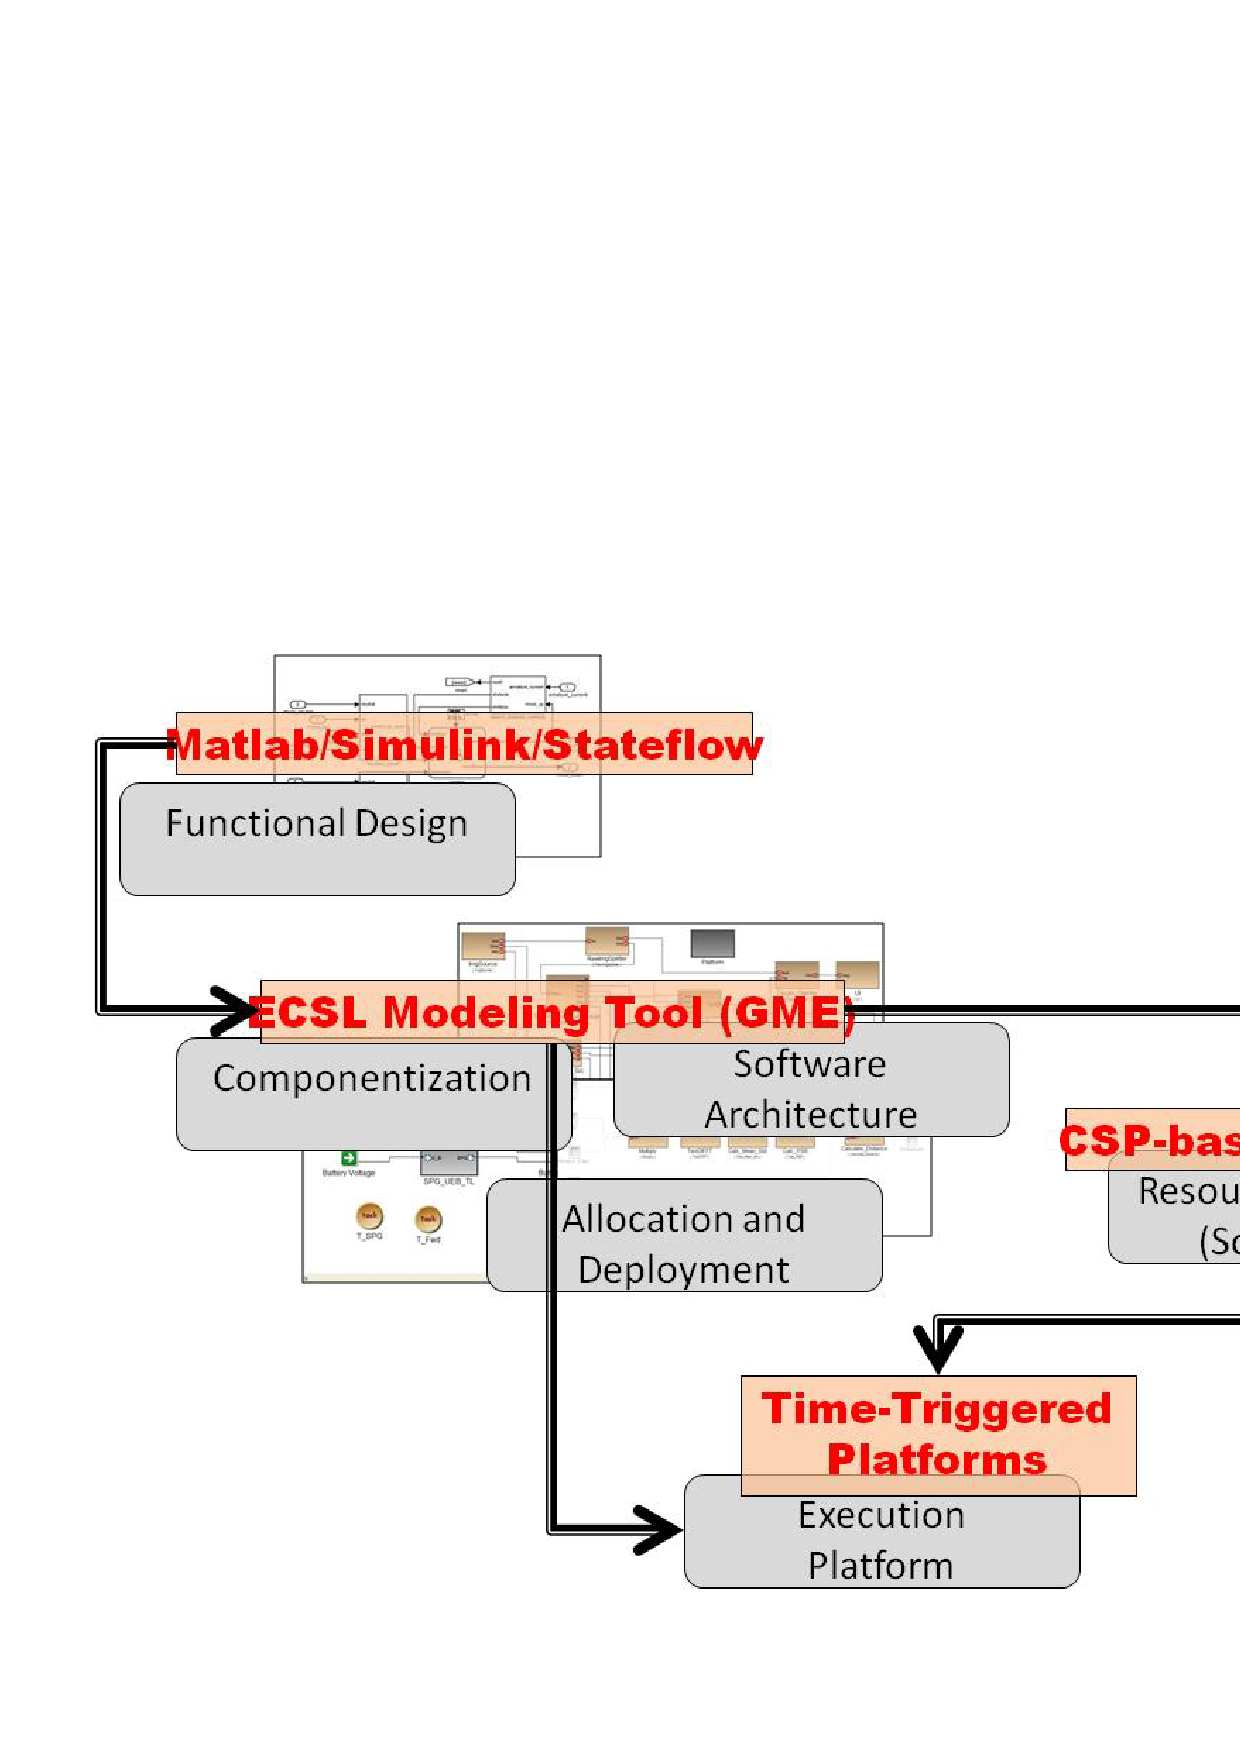
\includegraphics[width=0.9\columnwidth]{existing}
   \caption{Existing elements of the toolchain.}
   \label{fig:existing}
\end{figure}

%-------------------------------------------------------------------------
\SubSection{Platforms}
The carefully chosen set of target platforms have great impact on
the design of the proposed toolchain. This will remain so in the future as we further refine the
design environment---particularly the feedback mechanisms from the
deployment stages. Based on our
initial experience with various platforms, we recognize two
fundamentally different computational models in the task scheduling
and communication domains. We believe that many of the practical
distributed embedded environments can be described by a
combination and blending of these models.

Event-triggered (ET) real-time systems are driven solely by the
occurrence of various events, e.g. the reception of a message, the
assertion of an external interrupt line, or a timeout. In this
computational model, the system responds to these events as
soon as possible, resulting in a very flexible but highly
unpredictable environment. A notable purely event-triggered distributed embedded platform is TinyOS \cite{tinyos}.

In stark contrast to event-triggered systems, time-triggered (TT)
systems generate control signals with the progression of a
system-wide global time over a static schedule defined in
the design phase. These control signals might trigger the sending
and receiving of messages, the activation of application tasks, or
mode changes.

One of the most important conclusions we reached in the early stages
of the project was to separate the communication models and task
scheduling models on the target platforms. This enabled us to mix
and match these approaches and provided the flexibility to
characterize real-world embedded execution platforms. The
interactions between these models and domains are an interesting and
important research area \cite{ucb:ptolemy2}; however, in the
prototype version of the proposed toolchain, we focused on the time-triggered scheduling and communication aspects of the target
platforms.

Although these platforms differ in their implementation of the time-triggered approach---later sections will detail these
differences---all follow some general rules and use similar
concepts. We support a general TT component model in the modeling
language we developed, called ECSL-DP. According to the TT model,
the timeline (both in the
communication and task scheduling domains) is divided into continuously
repeating periods. The task and message schedule describe the
partitioning of this period. The length of the periods for task
scheduling and for communication are of equal length but obviously
have different partitioning. Optionally, the period can be divided
into subperiods of equal lengths (hardware implementations of TTA function in this way). Both the communication
subsystem and task scheduler wait for the beginning of the
period---in a synchronized manner---and control access to the
communication medium and/or release tasks according to a predefined
schedule throughout the period. At the end of the period, the whole
process starts again.

\subsubsection{The Time-Triggered Architecture platform}

One of the experimental target platforms for the toolchain is the
Time Triggered Architecture \cite{kopetz:2001-22} developed at the
Vienna University of Technology and by TTTech Computertechnik AG.
The primary reasons for selecting TTA, in general, and the
TTP-Development Cluster as a test platform were its fault-tolerance features, performance characteristics, and its technological maturity.

Fault-tolerance is supported by redundant communication channels, by
replicated subsystems with constant state synchronization and
voting in the value domain, and by various provisions in the
communication protocol (e.g. cluster startup, distributed time
synchronization, and membership management with clique avoidance). The
measured jitter, relatively high bandwidth, and protocol efficiency (low overhead)
are definitely superior to
similar performance metrics measured in general purpose (ET)
computer systems. However, one of the most crucial advantages of the Time-Triggered Platform (TTP)
for the system designer lies in its composability aspects. A
well-designed cluster schedule (with enough spare capacity for
future growth) guarantees that existing services are not affected by
the removal or the addition of other services both in the value and time domains. Furthermore, due to the dedicated and
autonomous protocol controller, these changes are transparent to the
application level software. Also, for similar reasons, application
level errors are not propagated to other nodes and do not disrupt
the communication channels.

These characteristics made the TTA platform and TTP prime targets for the proposed toolchain . On the other
hand, we faced various constraints and peculiarities inherent
in the TTP protocol, some of which had profound effects on the system
design and on the design environment. These lessons confirmed the need for an integrated environment,
where (late) deployment decisions are able to influence the (early)
design phases via feedback in the toolchain. This section gives a
brief overview of the protocol to illustrate some of the special
characteristics of TTP and their effects on the system
design.

In TTP all protocol operations, except during the \emph{startup}
phase, are initiated at \emph{a priori} known points in time. All
nodes that are integrated in the cluster agree on a global time. This
requires synchronized clocks with a fault-tolerant
synchronization protocol. The global clock is defined in a
\emph{sparse time base}, in which granularity is limited by the
precision of the distributed clock synchronization. The granularity
factor ($\Pi$) is an important parameter in the system design and
depends on the accuracy of the local oscillators, the frequency of
the synchronization points (TTP does not use skew compensation
techniques), on the speed of the communication controller, and the
physical medium. The communication controller has complete knowledge
of the message schedule---defined in a special descriptor table
located in the memory of the controller---and provides a shared
memory interface for the host processor to access the messages to be
sent and received.

The message schedule defines a \emph{cluster cycle}---or multiple
cluster cycles if cluster mode changes are allowed---which is
executed periodically (see Figure~\ref{fig:TTPSchedule}). The
cluster cycle is further divided into \emph{TDMA rounds}. Within a
TDMA round each node is assigned to exactly one slot---a time
interval where it can send messages packed into a single frame on
the communication bus. The length of these slots may differ for
different nodes, but they are constant throughout the TDMA rounds in the
cluster cycle (thus the length of the TDMA rounds are of the same
length in the cycle). Mode changes may alter the length of the
cluster cycle (the number of rounds in a cycle) and the message
contents of the frames, but the same ordering and lengths
of the time slots for the nodes should be used. These spartan scheduling rules make
mode changes and scheduling more deterministic and easier to handle,
but they have crucial effects on the system design. In a typical TTP
application, the length of the TDMA rounds are around 1-2~ms and the
precision of the synchronization is below 5~$u$S (re-synchronization
occurs at the end of each round). However, the number of rounds in a cycle
varies substantially, as do the length and contents of the frames.

\begin{figure}[h]
   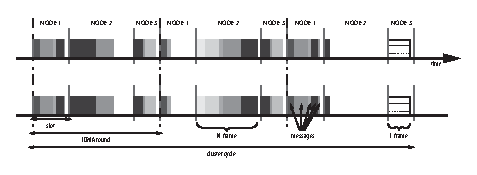
\includegraphics[width=3in]{TTPSchedule}
   \caption{Message scheduling in a TTP application.}
   \label{fig:TTPSchedule}
\end{figure}

The application design on the TTP platform may follow two different
approaches. In the simpler case, the application level tasks are not
synchronized to the communication bus, and tasks access the messages via
the shared memory interface as they wish. This approach has obvious
limitations (no guarantees on end-to-end jitter and latency) and can
hardly be considered real-time. More interesting is the second
alternative, where application tasks are activated in sync with the
message schedule. To support this method, the communication
controller provides interrupts to the host processor at well-defined
time instants while executing the protocol. The real-time operating
system running on the host processor is able to align the task
schedule with the bus schedule. Evidently, the limitations on the
message schedule affect the task schedule also in these systems. The
application cycle has to follow (match in its length) the cluster
cycle. Also, tasks cannot be released before the arrival of their
input message(s) and must finish before the transmission of their
output(s). Furthermore, fault management for subsystem replication
(tolerance against faults in the value domain) is implemented as
higher level services running on the host processor, thus additional
tasks and their dependencies have to be considered in the
application design. The task schedule with its important
dependencies in a typical application is shown in
Figure~\ref{fig:TTPAppSchedule}.

\begin{figure}[h]
\begin{center}
   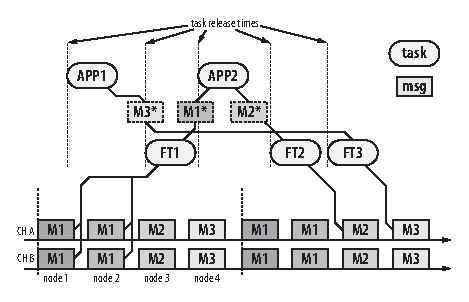
\includegraphics[width=3in]{TTPAppSchedule}
   \caption{Message scheduling in a TTP application.}
   \label{fig:TTPAppSchedule}
\end{center}
\end{figure}
\subsubsection{The FRODO platform}

Although the TTA approach to fault-tolerant execution of control applications has been developed and matured over many years, its current manifestation only as a hardware specific platform restricts the flexibility and portability of possible applications developed using the toolchain.  These obstacles motivated a second deployment platform for the toolchain that offered the same deterministic execution of the TT MoC with off-the-shelf components and a hardware/software independent platform API.  The resulting platform uses an abstract virtual machine, called FRODO, for executing TT control tasks of high-confidence systems coupled with a message controller that provides the TT transmission of data message across networked nodes, all of which is implemented using readily available infrastructure.

\subsubsection*{Architecture}

This platform's implementation architecture is based on logical separation principles similar to those of other TT platforms like Giotto \cite{henzinger01giotto} and TTA \cite{kopetz:2001-22}:  the periodic execution of control tasks is determined solely by the passage of time and the current operational mode of the system, i.e. events such as the arrival of new data messages do not affect the timely task execution.  Accordingly, only the most recent data values, representative of some control signals, are relevant to calculations performed by TT tasks; therefore, a globally shared memory construct is used to read and update data throughout execution.  The resulting architecture is provided below in Figure~\ref{fig:FRODOArch}.  In the figure, bidirectional arrows represent the flow of data throughout the system whereas the unidirectional arrows indicate the sending of relevant events.  The current platform implementation uses embedded PC-s running on Linux 2.6.x kernels and standard Ethernet UDP network for communication.

\begin{figure}[h]
  \centering
   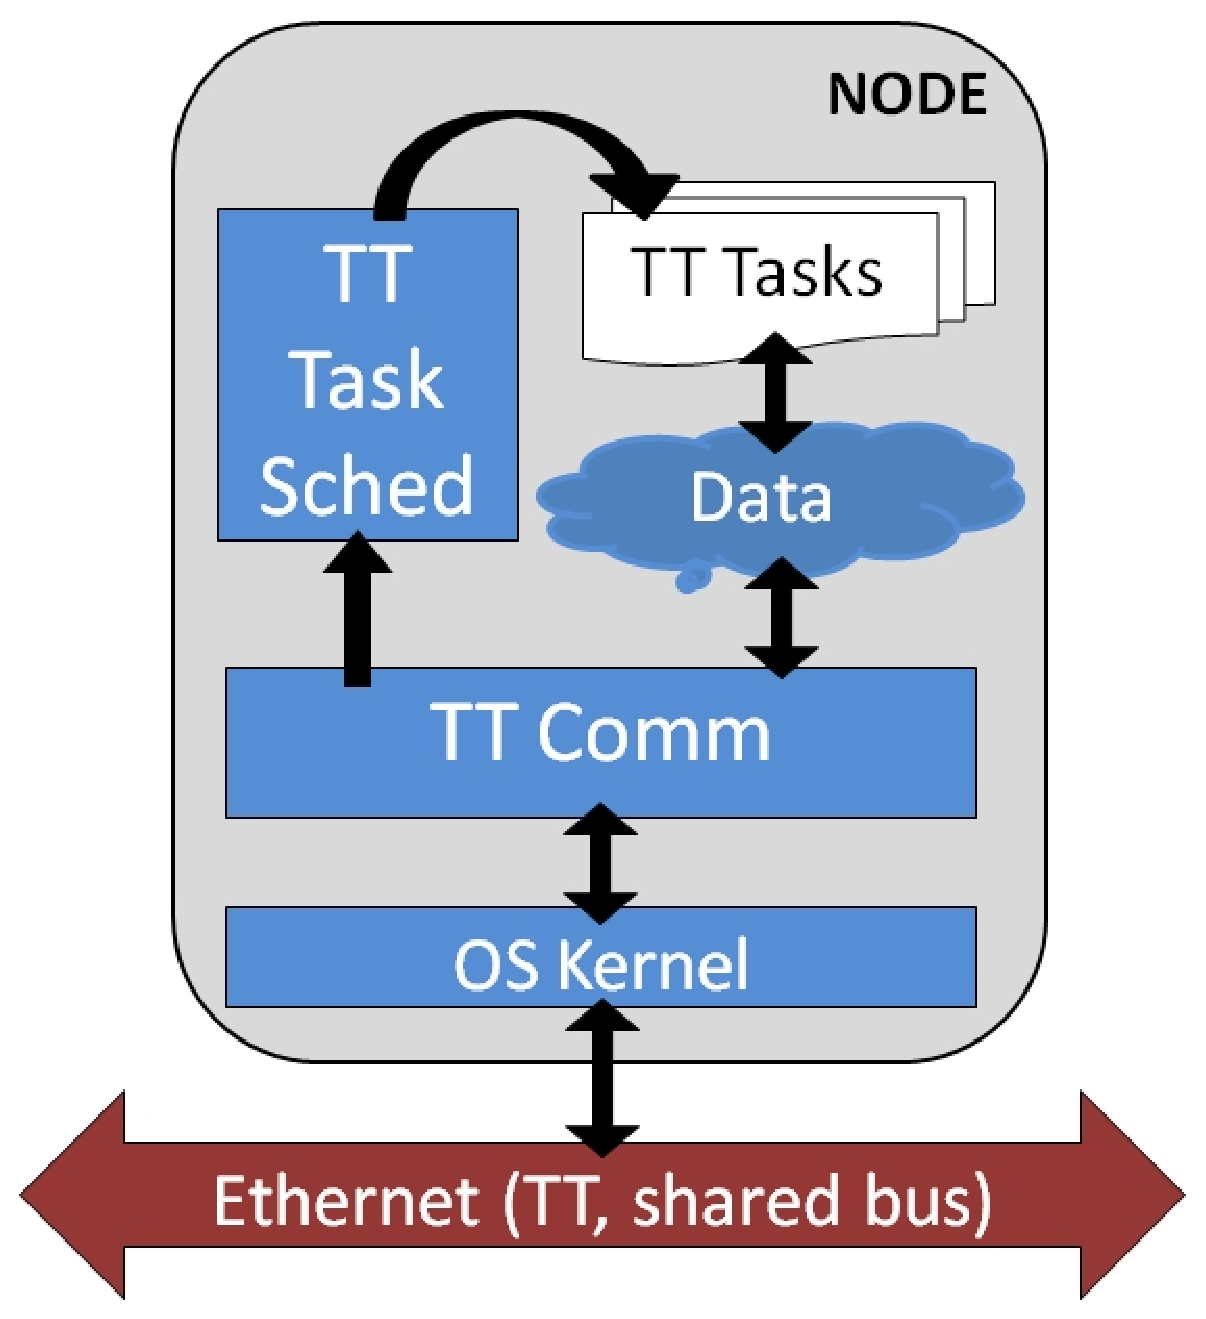
\includegraphics[width=0.5\columnwidth]{FRODOArch}
   \caption{FRODO implementation architecture.}
   \label{fig:FRODOArch}
\end{figure}

\subsubsection*{Time-triggered communication}
Maintaining low overhead and platform independence for the message controller was necessary to making this platform as portable as possible.  Accordingly, the communication controller expects only a shared bus network configuration for connecting all of the nodes in the system and a library of methods that provide the basic functionality for sending and receiving messages.  Unlike the TTP platform described above but similar to the TTP/A protocol \cite{kopetz:2000-23}, this platform is not yet robust enough to provide a fault-tolerant synchronization approach for maintaining a global clock; instead, a designated communications controller in the system is responsible for initially verifying all of the expected nodes are connected to the network before starting execution and synchronizing the start of the each message schedule round with all of the nodes.  All other nodes on the network will not begin executing unless confirmation is received that all nodes are present at startup, and they will also fail to start a new schedule round unless the proper synchronization message is received.

Based on the previous discussion of the properties of the TT MoC, the certification/verification of distributed control systems is contingent upon the deployed system's ability to accurately follow a fixed message schedule; therefore, the use of a TT capable message controller is paramount to this platform's applicability for systems developed using the toolchain.  Like the TTP approach, a static message schedule is generated offline, passed as an input to the platform, and cyclically iterated throughout the execution; however, the format of the message schedule is not identical to that used in TTP.  TTP requires the use of a strict TDMA format where all nodes have a scheduled time-slot for transmitting messages in each round.  Conversely, this platform does not place any minimum or maximum on the amount of data that can be sent from a node in a round except those constraints that maintain the feasibility of the message schedule.  Instead, the static message schedule specifies exactly which node sends a message at an exact scheduled offset with respect to the start of the schedule round.  Each schedule round is one hyperperiod long, and the hyperperiod is of fixed duration.  A node will be allotted no messages/slots if it is not expected to transmit any data within a schedule round.  If a message is expected to be sent with a frequency greater than one within a round, it will be listed as many times in the schedule as it is expected with each appropriate scheduled transmission time.  The length of each message, in bytes, is also indicated in the message schedule.

The current steps for establishing and maintaining TT communication across a network of nodes implemented using this platform proceeds in the following steps:
\begin{enumerate}
\setlength{\itemsep}{1pt}
\setlength{\parskip}{0pt}
\setlength{\parsep}{0pt}
\item Discovery of all nodes required by the implementation
\item Transmission of hyperperiod start signal (beginning of schedule execution)
\item Transmission of data messages in their strict scheduled order
\item End of hyperperiod is reached
\item Repeat starting from step 2 or terminate execution
\end{enumerate}
Obviously, while each individual node is preparing to transmit its scheduled data messages, it must also be configured to receive broadcast messages from other controllers in order to maintain the most up-to-date data set.  Each outgoing message includes a message indicator such that the receivers can quickly locate the appropriate memory location to update with the received value.  A snapshot of the activity on the communication network over two hyperperiods of the message schedule is provided in Figure~\ref{fig:FRODOTimeline}.

\begin{figure}[h]
   \centering
   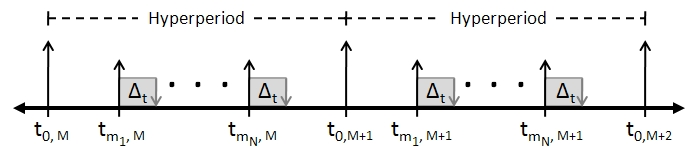
\includegraphics[width=0.95\columnwidth]{FRODOTimeline}
   \caption{Activity timeline across time-triggered network.}
   \label{fig:FRODOTimeline}
\end{figure}

\subsubsection*{Time-triggered task execution}
The application code that provides the functionality of the individual toolchain components is generated completely agnostic to the choice of target platform(s).  Instead, the tasks that contain the application code of the components provide only timing information regarding their execution and require access to the data relevant to the control calculations they perform.  Accordingly, the platform's task scheduler need only expose an interface fitting the tasks' needs and have the capability to invoke and terminate task execution in order to provide precise controller execution.  FRODO is such an abstract, platform-independent executive (virtual machine) responsible for providing the necessary TT execution of control tasks on this platform.

Most commonly, digital implementations of controllers operate in a periodic fashion---sampling control signals, computing the next control signal and the current state of the system, and performing an actuation based on the computations.  Likewise, the task scheduler of FRODO is responsible for initiating the periodic execution of the control tasks based on a static task execution schedule initially passed as input to the system.  The current implementation of FRODO does not allow the preemption of tasks, i.e. only one periodic control task is released for execution at any given time.  In order to maintain the timely execution of the control tasks according to the schedule, FRODO is also responsible for terminating executing tasks that have yet to finish prior to reaching their worst-case execution time (WCET).
The task schedule for a node is similar to the message schedule mentioned in the preceding section: each task invocation is explicitly listed in the schedule with its appropriate release time with respect to the start of the schedule and the task schedule has the same length or hyperperiod as the message schedule.  Synchronizing the execution of the task schedule with the message schedule maintains the controller correctness with respect to the current control signals; therefore, each new round of the task schedule has to be initiated by the arrival of an event from the underlying communication controller indicating that a new schedule round is beginning.  If no such event is received, the control tasks will not be released for execution.

Only as a scheduled task begins and (properly) ends execution, it will require the necessary access to the globally shared memory to read/update the control signal data used throughout the system.  Accordingly, FRODO provides two methods for performing such operations; however, internally FRODO must use proper access-control locks to ensure that it is not updating values concurrently with the message controller.


\SubSection{Modeling languages}
As described earlier, graphical modeling languages and transformations bind together functions of the toolchains.  These languages are defined using metamodels in the Generic Modeling Environment (GME) \cite{isis:gme}, which is also used directly to edit models thus represented.  Graph transformations are specified using GReAT \cite{isis:great}.  These generic tools aim to provide the necessary framework to enable an end-to-end development solution: from functional design using Simulink/Stateflow, through verification of critical operational properties, down to certified code that can be used confidently on the specified platform.  Here we describe details of the modeling languages in the tools and the intended design flow.

In a typical design, a control designer will capture physical models mathematically, and then represent them in a simulation tool such as Simulink.   Controllers are then specified by adding dataflow model elements to the Simulink model, possibly with state-based controller elements specified in Stateflow. Implementations of the controller functions may be generated in C code using Real-Time workshop, or written by hand.  Next, the implementation must be pasted into a software design framework, which was likely created using UML tools.  Testing and debugging follow, then  final deployment.

Envision instead a tool that imports Simulink and Stateflow models directly into a model-based software design environment.  Within this environment are additional modeling languages that describe software component partitions and interfaces, as well as hardware descriptions.   ECSL-DP (Embedded Control System Language for Distributed Processing) is an aggregate language that includes all of these constructs \cite{KS:ISIS-04-505}. Figure \ref{fig:packages} depicts the elements of the language.  The components, platform, and mapping languages of ECSL-DP will be described here, with highlights of important constructs.

\begin{figure}[h]
\begin{center}
   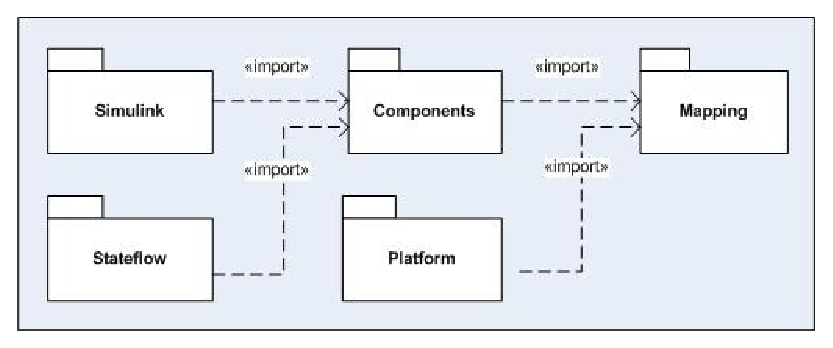
\includegraphics[width=0.9\columnwidth]{packages}
   \caption{Relationships between sublanguages in ECSL-DP.}
   \label{fig:packages}
\end{center}
\end{figure}

\begin{figure}[h]
\begin{center}
   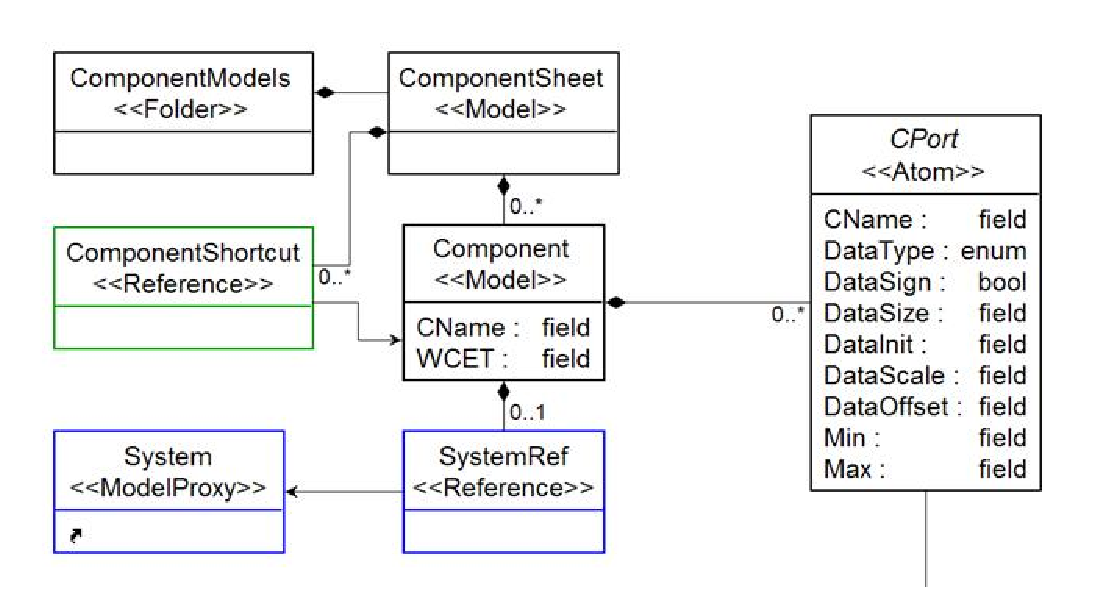
\includegraphics[width=0.9\columnwidth]{component_meta}
   \caption{Fundamental elements of component models in ECSL-DP.}
   \label{fig:CompMeta}
\end{center}
\end{figure}

Figure \ref{fig:CompMeta} illustrates the basic elements of the modeling language for describing the allocation of Simulink blocks to software components.   Components refer to Simulink Systems, and have ports (interfaces) for exchanging data.  The meta-programmable modeling environment allows us to extend the language with particular concepts, such as real-time execution time constraints as shown in Figure \ref{fig:RealTime}.  This modeling construct is not currently used by the code generators, but illustrates the extension mechanism for adding future capabilities.

\begin{figure}[h]
\begin{center}
   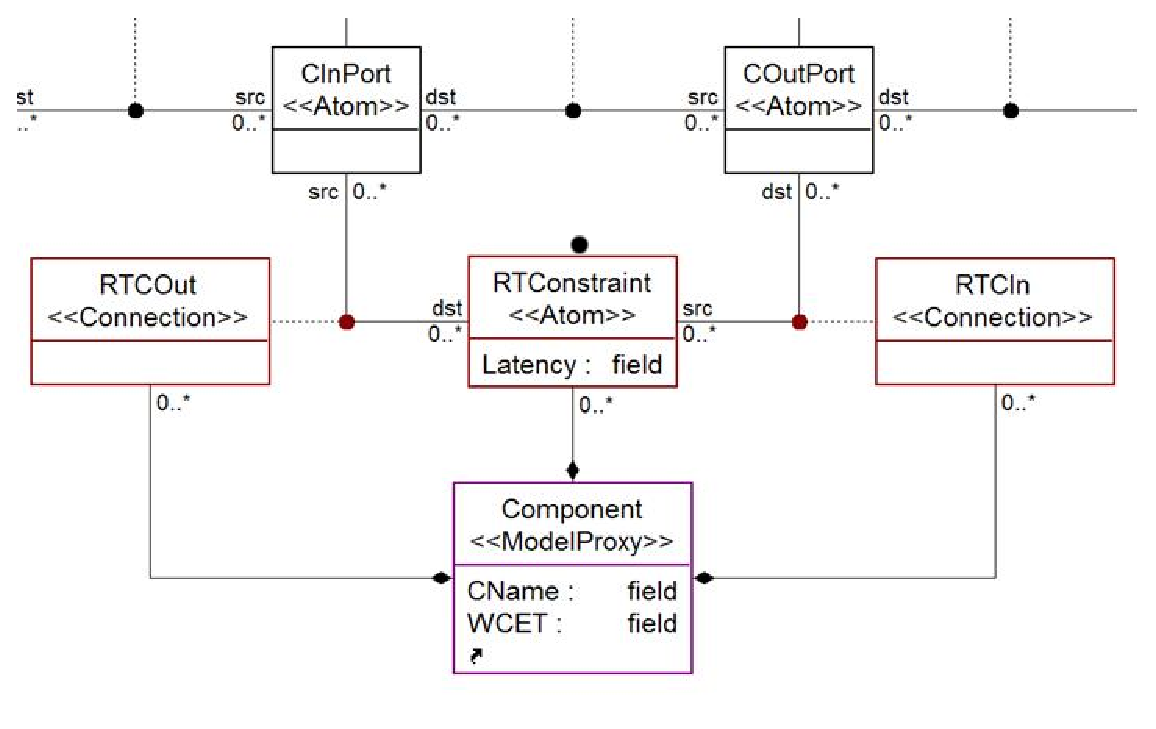
\includegraphics[width=0.9\columnwidth]{real_time}
   \caption{Real-time execution constraint models for components in ECSL-DP.}
   \label{fig:RealTime}
\end{center}
\end{figure}

The key parts of ECSL-DP provide the most benefit over alternative code-generation schemes.  In ECSL-DP hardware platforms are modeled directly, and then the component architecture is mapped onto the hardware topology using graphical modeling tools.   Hardware models are simple networks of processing elements and communication buses.  Model parameters include data transfer rates and other essential configuration items.  Figure \ref{fig:MappingMeta} shows metamodel elements for this mapping.  The modeling languages for platforms and components are composed to form a new sublanguage within ECSL-DP, which precisely defines the relationship between concepts in both languages.  Software components are assigned to tasks, which are assigned to run on a single processing element.  Tasks specify the period of cyclic execution.  The mapping also defines communication messages for connected buses, and relates them to communication ports in the component model.

\begin{figure}[h]
\begin{center}
   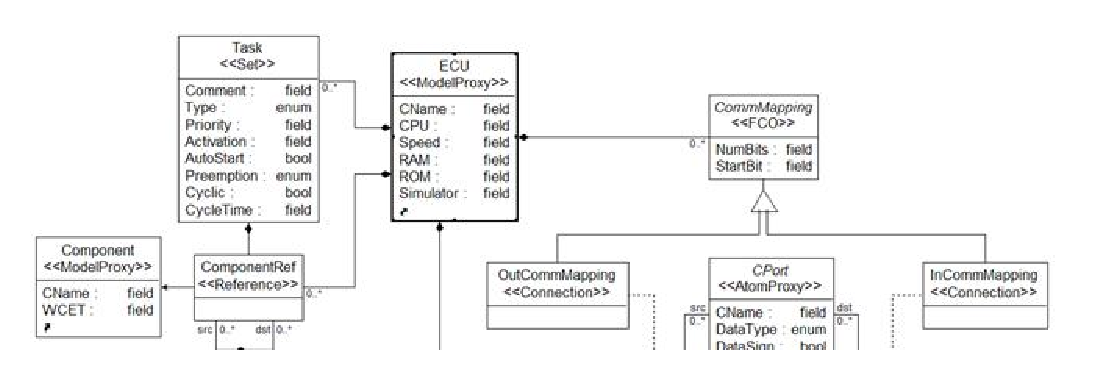
\includegraphics[width=0.9\columnwidth]{mapping_meta}
   \caption{Metamodel for mapping software components to platform elements.}
   \label{fig:MappingMeta}
\end{center}
\end{figure}
     
     In summary, consider the different aspects of the model:  Start with functional blocks connected by signals; These are wrapped, respectively, into components and their associated communication channels, which are mapped (respectively) to tasks on processors and messages on buses.  The resulting layered model captures all of the necessary information to generate code, create time-triggered schedules, and configure the platform.  These functions are currently available in the toolchain, and they are implemented using model interpreters and graph transformations, described below.  The next steps in tool evolution will add verification concepts at different stages of the design and integrate the proper tools to enable safety-assured software designs.


\SubSection{Generators}
%-------------------------------------------------------------------------

% SL_CodeGen functions, prototypes, datatype mapping to C, classes (instances), primitives and supported data types on signals (table?) (example SFC model and source code)
% GReAT and other implementation details
% SF_CodeGen how SL and SF "meet", functions and classes (instances)

\subsubsection* {General Discussion}

The main role of the code generators in the proposed toolchain is to transform the dataflow and statechart models into executable code
on the selected hardware/software platform as it is described by the component and deployment aspects of the ECSL-DP model. Currently, different generators exist in the toolchain for the different parts of the model, and the final compilation and linking step combines the generated artifacts. The SDF and HFSM code generators are the key components of the code generation infrastructure, and they share their internal architectures and underlying technologies. Both tools are built using the GReAT engine \cite{isis:great}, and they employ graph rewriting rules on the dataflow and statechart models to transform them into an intermediate model-based representation of the executable code.  This approach has benefits. The heavyweight part of the code generation is decoupled from the concrete syntax of the platform language (in this case C or C++); consequently, it is remarkably straightforward to add support for additional procedural languages. Also, the model-based representation of the generated code (in the form of abstract syntax graphs) provides a clear and well-defined programmatic interface to the generated code for verification tools or other third party utilities.
Although the proposed toolchain elements are built on strict and formal graph transformation foundations, the code generation infrastructure shows many similarities to the overall approach taken by the GNU Compiler Collection, which partitions the compiler workflow into front-end and back-end systems with the Register Transfer Language intermediate representation between these \cite{gcc}.

\subsubsection* {Synchronous Dataflow code generator}

The Synchronous Dataflow (SDF) code generator (\emph{SL\_CodeGen}) performs a topological sort on the input dataflow model before it executes the transformation rules which finally yield executable code. Signal paths become variables and dataflow blocks are transformed into functions. The code generator is prepared to handle many of primitive processing elements and automatically generates their implementation in the given context. The following Simulink blocks are supported currently: {\tt Product, MultiPortSwitch, Constant, Signum, Sum, ToWorkspace, Math, BusSelector, Mux, RelationalOperator, Demux, UnitDelay, Terminator, Gain, Saturate, MinMax, Switch, Ground, From, Goto, Abs}

The internal architecture of the code generator makes it rather straightforward to add support for other blocks in the future. Scalars, vectors, matrices and structures are supported on the signal paths.

\subsubsection*{Hierarchical Finite State Machine code generator}

The Hierarchical Finite State Machine (HFSM) code generator processes imported (sub)models from Stateflow language. Thus, it follows the semantics of a subset of MATLAB/Stateflow \cite{mathworks:tools} as closely as possible while generating the executable implementation. It employs sequential evaluation semantics for state transitions. The transitions are evaluated on the state hierarchy with a depth-first search for active states. A state transition into a new state implicitly enters all of its parent states. Like in MATLAB/Stateflow, the code generator assigns three functions for each state: one for executing actions upon entering the state, another for the exit actions, and a third one for performing tasks while the state is active.

\subsubsection{TTP code generator}
The Time-Triggered Platform presented several challenges to the creation of code
generators. It has intricate constraints on the task and message
schedules, and the message schedules are not contained by the
application code but by a special message descriptor file (MEDL), which
is downloaded to the controller at startup. Due to the closed source
model of the TTP software toolset, we faced an important decision in
supporting this platform. We either had to replicate (some of) the
functions of the TTP tools or somehow integrate them into our toolchain.
For the first prototype the second approach seemed to be more
reasonable. Each of the TTP tools provide a Python-based API for
automating the design process. These APIs proved to be rich enough
to integrate the tools into the prototype toolchain. The \emph{TTP
Code Generator} is responsible for the following steps:\\
\textbf{Glue code generation.} The deployment model of the ECSL-DP
  language defines the tasks and the contained software
  components. The software components refer to Simulink blocks
  in the dataflow model. The TTP code generator is responsible
  for generating the "body" of the time-triggered tasks that read
  the input variables, invoke the functions generated
  by the Simulink/Stateflow code generators, and update the
  output variables in the communication controller. The
  generated glue code is also responsible for the cluster
  startup and the re-integration of tasks after failures.\\
  \textbf{Message scheduling.} In parallel with the code generation
  steps, the TTP code generator builds a Python script as an
  input for the \emph{TTPplan} tool. The generated script
  defines the global properties of the cluster, the messages,
  their types and required frequencies, the nodes, and a default
  cluster mode. The source of this information is the deployment
  model.\\
  \textbf{Task scheduling.} The code generator also builds Python
  scripts for the \emph{TTPbuild} tool---one for each node. The
  script defines the application level tasks (based on the
  deployment model) with their worst case execution times and builds
  the connection to the input and output messages.\\
  \textbf{Compiler execution.} Finally, the TTP software tools are
  executed with the generated script files. TTPplan generates
  the message schedule (if the scheduling requirements can be
  satisfied). TTPbuild customizes the MEDL for each node,
  generates a configuration file for \emph{TTPos}---a real-time
  embedded operating system running the cluster nodes---and generates the
  source code for the fault-tolerant communication layer.
  Provided that the previous steps succeeded, the TTP code
  generator invokes the compiler on the generated source files
  (Simulink/Stateflow code, TTP glue code, fault-tolerance layer,
  and operating system configuration).\\

\subsubsection*{Constraint-based scheduler}
% What it does
Commercial TTP tools provide deployment analysis and schedule generation capabilities subject to use on a particular hardware platform.  Our toolchain includes a more general schedule generation tool that can create time-triggered schedules for tasks and messages in a distributed system.  A GReAT transformation extracts the critical details from an ECSL-DP model and models them in a simple system description language called \emph{CSched}.  \emph{CSched} includes system description models, instance graph models, and constraint program models.  Once the system model is created using the graph transformation, the system and constraint models are automatically created by a model interpreter.  Constraint models are solved using the finite-domain constraint library Gecode \cite{gecode}.  Any feasible solution represents a valid schedule for all tasks and messages in the system. Constraint-based schedule generation has been shown to scale well to large problem sizes.  Schild and W\"urtz report successful scheduling of up to 3500 processes and messages, 1 million constraints, and a search space dimension of 6 million starting times \cite{sw:offlinescheduling}.

% How it does it
The difficulties of representing TTA scheduling problems as finite-domain constraint models lie in capturing the variations of order that can occur among the task and message instances and in attempting to optimize the orderings to satisfy specified latencies.  Schild and W\"urtz \cite{sw:offlinescheduling} describe a two-stage modeling technique for this problem: in the first stage, task and message dependencies are resolved and the resulting execution order is captured in constraints; in the second stage, the constraint space is searched to satisfy latency constraints within the established ordering.  Our approach simplifies this technique by using additional global serialization constraints to represent the families of task/message orderings in an attempt to reduce solution effort to a single stage.  This work is still in progress, but the tools do produce valid schedules for many configurations and are fully integrated into the toolchain.

%-------------------------------------------------------------------------


\Section{Related work}

\section{Related Work: Languages and Tools for Embedded Systems Design}

A number of projects seek to bring together 
tools and techniques which can automate different
aspects of high-confidence distributed control system design and analysis:

\begin{itemize}

\item AADL is a textual language and standard for 
specifying deployments of control system designs in data 
networks\cite{modeling:aadl_control_systems}.  AADL 
projects also include integration with the Cheddar 
scheduling tool\cite{sched:aadl_sched}. Cheddar is 
an extensible analysis framework which includes a 
number of classic real-time scheduling 
algorithms\cite{sched:cheddar}.

\item Giotto\cite{modeling:giotto3} is a modeling 
language for time-triggered tasks running on a single 
processor.  Giotto uses a simple greedy algorithm to 
compute schedules.   The TDL (Timing 
Definition Language) is a successor to Giotto, and 
extends the language and tools with the notion of 
modules (software components)\cite{timed:tdl}.  One version 
of a TDL scheduler determines acceptable communication windows 
in the schedule for all modes, and attempts to assign bus 
messages to those windows\cite{timed:tdlflexray}.

\item The Metropolis modeling framework\cite{modeling:metropolis} 
aims to give designers tools to create verifiable system models.  
Metropolis integrates with SystemC, the SPIN model-checking tool, 
and other tools for schedule and timing analysis. 

\item Topcased\cite{tools:Topcased} is a large tool integration effort
centering around UML software design languages and integration of
formal tools.

\item Several independent efforts have used the synchronous 
language Lustre as a model translation target 
(e.g. \cite{modeling:lustre2} and \cite{modeling:lustre1}) 
for deadlock and timing analysis.

\item RTComposer\cite{modeling:rtcomposer} is a 
modeling, analysis, and runtime framework built on 
automata models.  It aims to provide compositional 
construction of schedulers subject to requirements 
specifications.  Requirements in RTComposer can be 
given as automata or temporal logic specifications.  

\item The DECOS toolchain \cite{modeling:decos} 
combines a number of existing modeling tools (e.g. the 
TTTech tools, SCADE from Esterel Technologies, 
and others) but the hardware platform modeling 
and analysis aspects are not covered.

\end{itemize}

We are creating a modeling language to experiment with design decoupling 
techniques, integration of heterogeneous tools, 
and rapid analysis and deployment.  Many of the 
listed projects are too large to allow 
experimentation with the toolchain structure, and 
standardization does not favor experimentation 
with syntax or semantics.  Due to its experimental nature 
some parts of our language and tool infrastructure 
change very frequently.  As functionality expands we 
may seek integration with existing tools or standards as appropriate.




\Section{Future work}
As this research effort is a work in progress, we conclude with a brief summary of
the next steps and future objectives for each of the tools presented.   We must 
keep in mind the final goal of verifiable and certifiable software for embedded 
systems.  This section contains forward-looking statements.

\SubSection{Software architecture specification}
The chief limitation of our software architecture tools is the one-way design flow 
from the SL/SF design, through componentization, down to the final 
code. We aim to improve the ability to send design information back to the earlier 
stages of the design as neeeded.  For example, platform-specific simulations may
indicate that jitter or quantization effects will impact the initial assumptions
of a control design.  Representing that data to control designers in a meaningful 
way will allow design changes without excessive workflow iterations.  
Schedulability is another area where downstream software 
design tools can provide meaningful feedback to the original design engineers.

\SubSection{Code generation}
The abstract model in the code generator opens the door for a number of
potential static analysis and verification opportunities.  The current toolchain 
includes two code generators that produce C (and Java) source code from 
(single-rate) subsystems in Simulink and Stateflow models. The code generators have 
been implemented using graph transformation techniques, and they produce an AST from 
which the actual code is printed. To assist in system-level or functional code
verification the AST could be extended to carry over information from the original 
model, thus providing guidance for the source code-level verification tool 
regarding the original model from which the code was generated and its properties.
We believe this can significantly improve the performance of the verification step 
because the verifier does not have to �reverse engineer� the high-level 
abstractions from the source code, as the abstractions are readily available in
the models. 

\SubSection{Scheduling}
We aim to expand the scheduling tools to include specific time-triggered models.
One simple example is that of adding constraints to support the requirements of
the TTTech TTP/C hardware.   Another avenue for research is the exploration of 
interactions between the resource allocation model (via schedules) with other 
system objectives which can be modeled by constraint or optimization problems in
other domains (such as continuous stability in the control design).  

\SubSection{Extending the modeling of the execution platform}
The formal DEVS model is a big step towards providing guaranteed safety and 
performance in time-triggered control system designs.  DEVS also supports pure
event-triggered behaviors in addtion to timed models.  Experimentation with this 
capability will hopefully lead to a better understanding of the limitations of 
heterogeneous component interactions in our system designs. 

Platform simulation also opens up opportunities for exploration.  The TrueTime tool
suite from Lund University \cite{TrueTime} extends Simulink models with 
concepts for modeling distributed platforms, scheduling policies, and communication 
protocols.   TrueTime promises to help characterize behavioral changes due to the
distribution of functionality over networked processors.

\SubSection{Extending the capabilities of the execution platform}
As the capabilities of the formal models expand, we aim to extend our portable
VM implementation to manage heterogeneous behaviors.  The VM will also be ported
to other operating platforms, including diverse hardware and RTOSes such as QNX 
and uC-OS.  Different platforms provide different levels of assurance regarding
timing, determinism, and resource management.  These differences will need to be
reflected in the models.  New features may also be added to the VM as required to 
support interaction idioms such as remote procedure calls or rendezvous.  We may 
also require additional component services such as health monitoring, fault management, 
robust clock synchronization, or failover.  



\Section{Acknowledgements}
This work was sponsored (in part) by the Air Force Office of Scientific Research, USAF, under grant/contract number FA9550-06-0312.  The views and conclusions contained herein are those of the authors and should not be interpreted as necessarily representing the official policies or endorsements, either expressed or implied, of the Air Force Office of Scientific Research or the U.S. Government.
%-------------------------------------------------------------------------
\bibliographystyle{latex8}
\bibliography{rtas_2008}

\end{document}
